% ----------------------------------------------------------
\chapter{Machine Learning for Text}\label{cap:ml_text}

In this chapter, we present the essential concepts  to understanding the results and discussion from this work. It starts from the basic definitions related to \gls{ML} and \gls{TM},  and the challenges related to them. There is an explanation regarding definitions, techniques, and evaluation of the three tasks applied during this research: text representation, text classification, and text regression. 
Finally, there is an explanation of pipelines for \gls{ML}.

%%%%%%%%%%%%%%%%%%%%%%%%%%%%%%%%%%%%%%%%%%%%%%%%%%%%%%%%%
\section{Basic definitions} \label{sec:basic_definitions}

%%%%%% ML  %%%%%%

% What is ML?
According to \textcite{Mitchell1997}, \gls{ML} is a sub-field from \gls{AI} and focuses on constructing computer systems that learn to perform tasks through experience. For \textcite{Samuel1959}, \gls{ML} is the field that focus on building systems which can learn to solve problems without being explicitly programmed. Such systems can learn to classify texts, control robots, predict weather, and others~\cite{Sebastiani2002, Kober2013, Shi2015}.
 
% Deep Learning
A sub-field of \gls{ML} is \gls{DL}, which brought improvements, achieving \gls{SOTA} results on the solution of problems in several areas, such as \gls{NLP}, Image Classification, and others \cite{Brown2020, Tan2021, Sengupta2020}. In addition to those relevant results, humans have been outperformed by \gls{DL} in complex tasks, like the Chess and Go games \cite{Silver2017}. 

According to \textcite{Lecun2015}, \gls{DL} techniques are representation-learning methods with multiple levels of representation. Starting from the raw input, the levels transform the representations until a more abstract level. 
% O que diferencia ML e DL
Thus, a relevant difference among  the Classical \gls{ML} and \gls{DL} techniques is the ability to deal with the data in its natural form, as in the former, the researcher needs to implement hard-coded feature engineering while in the latter, there is no such need. \gls{DL} techniques can learn more complex functions and tend to produce larger models, with more hyper-parameters.


ML based systems, both Classical and \gls{DL} can learn using some approaches \cite{Schmidhuber2015, Caruana1997}, including supervised and unsupervised. In supervised \gls{ML}, the system maps a relationship between inputs and outputs based on labeled data. In unsupervised ML, the system tries to find patterns in the data taking into account the similarities among the many date points~\cite{Theodoridis2009}.
Examples of supervised learning tasks include classification, and regression, and examples of unsupervised learning tasks include clustering and topic modeling \cite{Kowsari2019, Aggarwal2018, Russell2020}.

% ML Model vs ML Technique vs ML Task

In this work, terms related to \gls{ML} are frequently used, such as task, technique and model. It is important to clarify each of them. A task in \gls{ML} relates to \emph{what} the learning machine intends to do, i.e., the type of inference that is done based  on the problem and the data available \cite{Quintanilla2015}. 

Another terminology regards \gls{ML} techniques, which relate to mechanisms and algorithms that allow the machine to learn. For example, there are classification techniques like Decision Trees and Naïve Bayes, and clustering techniques such as K-means and Lingo \cite{Osinski2004, Aggarwal2018}. 
Based on a \gls{ML} technique,  and the data, the machine learns to perform a task during the process of \textit{training}. The result of such process is a \gls{ML} \textit{model}, i.e.,  the representation of the learned function \cite{Quintanilla2015}.

%%%%%% TM & NLP %%%%%
% What is TM?

Beyond \gls{ML}, an important field of study applied in this work is \gls{TM}. \gls{TM} relates, according to \textcite{Aggarwal2013},  to the idea of discovering and analyzing patterns, such as trends and outliers, from textual data. TM also focus on helping users to analyze and digest information towards a better decision making. Thus, the necessity of TM and ML based applications emerges with the large amount of textual data  generated by users, companies, universities and so on, and human limitations to analyze it~\cite{Lecun2015, Khan2014}. Examples of \gls{TM} tasks are text classification, text clustering, text regression and others \cite{Aggarwal2018}.

% What is NLP?
An important field related to \gls{TM} is \gls{NLP}, 
which employs computation techniques to process, learn, understand, and produce human language content. That is, they generally receive textual data as input and produce text as output  \cite{Hirschberg2015}.
Examples of \gls{NLP} tasks include text summarizing, \gls{POS} Tagging, text preprocessing, text translation, and text generation \cite{Gambhir2017, Brown2020}.

When applying \gls{ML} to texts, generally both \gls{TM} and \gls{NLP} may be used. To do so, one can build pipelines to aggregate these three and other types of techniques.

A \textit{pipeline} is an computational architecture composed of several processing units connected in sequence and each of them is responsible for a distinct processing computation \cite{Ramamoorthy1977}. 
%An important aspect of pipelines is the modularity of the units, which can be added, replaced, and removed without much effort.
In \gls{ML}, pipelines help on building complete systems which can receive raw data as input, preprocess it, train the models and evaluate their performances \cite{OBrien2021}.

In Figure \ref{fig:cap2_example_pipeline}, there is an example of \gls{ML} pipeline to text classification \cite{Kowsari2019}. 

\begin{figure}[htb]
    \centering
    \caption{Example of pipeline for text classification}
    \label{fig:cap2_example_pipeline}
    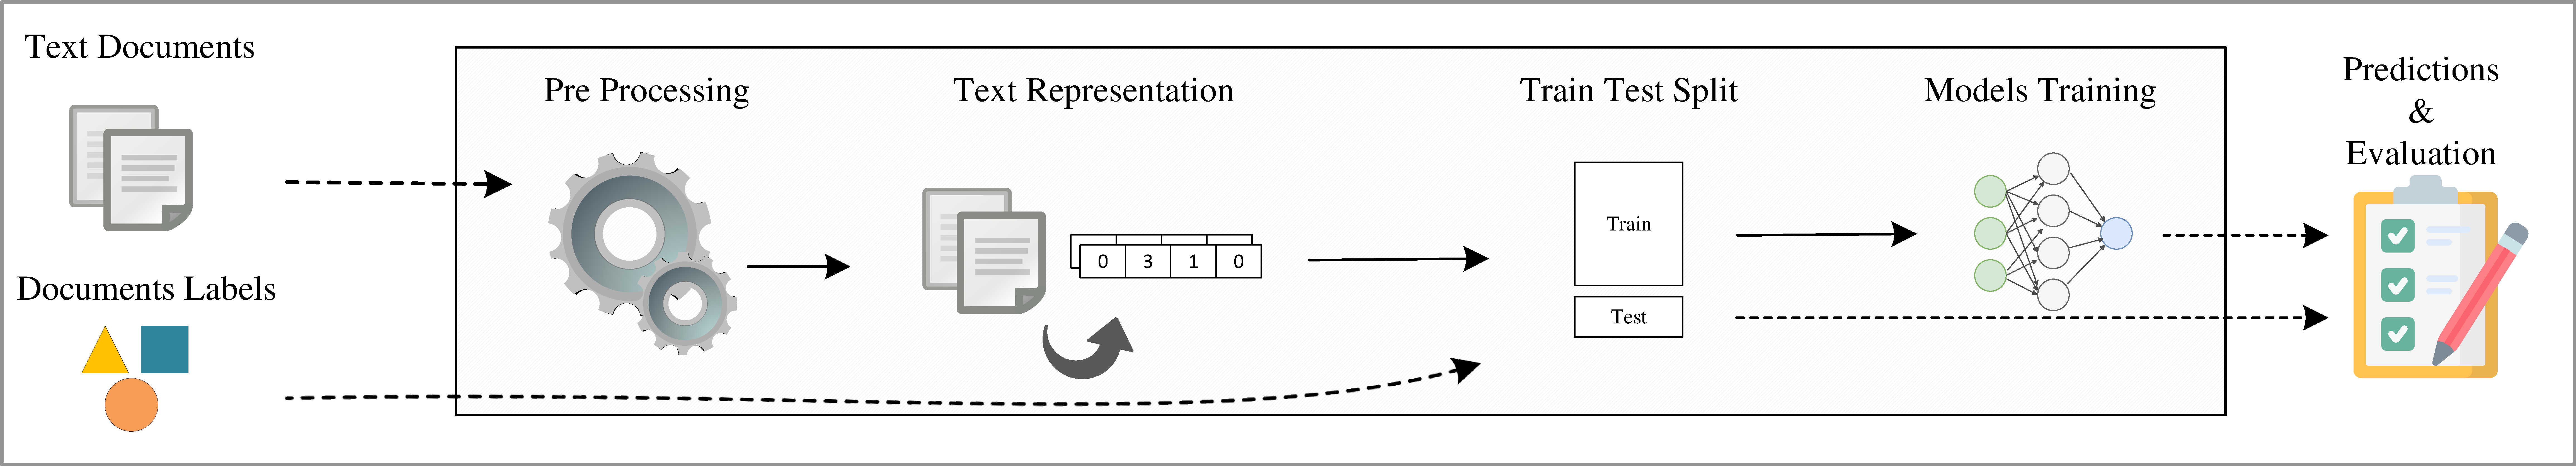
\includegraphics[width=\textwidth]{images/chapters/cap4_simple_pipeline_regression.pdf}
\end{figure}

It receives two types of inputs: the text from the documents and the labels. The data passes by some steps, starting by the pre-processing and the textual representation. 

To train the classification models, it is required the data and the technique. To evaluate the models, unseen data is required. Thus, the dataset may be split in train and test sets. Among the methods to do that there is the random sampling, which randomly selects instances in the dataset for the two sets, in proportions of 80\% and 20\%, respectively (70\% and 30\% is also used) \cite{Kotu2019}. 

Finally, the pipeline outputs the trained models and the test set for performance evaluation.


When dealing with supervised learning applications, one can face some difficulties to get good results~\cite{Alzubaidi2021,Kornilova2021}. 
One is the \textit{overfitting}. It occurs when the models are too specialized in the train data and they achieve a poor prediction quality when evaluated in the test set~\cite{Karystinos2000}. 
According to \textcite{Hawkins2004}, a model is overfitted when it achieves the same prediction quality when compared to a simpler one. Thus, the model is more complex than it should be. A possible adjustment to reduce overfitting is to reduce the complexity of the models, that is, check whether simpler models perform as well as the complex ones~\cite{Liu2016}. 

% Outliers
A further common challenge that can affect the learning task is the presence of outliers in the dataset. There may be instances very distinct or inconsistent from the others. These instances are called \textit{outliers}. Depending on the \gls{ML} technique, their existence in the dataset may degrade the prediction quality of the models~\cite{Freeman1995}. 
%So, we want to remove these examples from our dataset using some outlier detection technique. 
Among the existing algorithms for discovering outliers~\cite{Hodge2004}, there is the Isolation Forest. It is a simple and efficient technique that isolates the anomalies at the upper levels of random trees~\cite{Liu2008}.


The method used to split the dataset into training and test subsets can introduce some bias in the pipeline. The distribution of the examples may not be similar in those two subsets, specially in small datasets~\cite{Hawkins2004}. By evaluating the models several times using different and random train and test sets the prediction quality measurements could be more precise. In this case, $k$-fold cross-validation can be used, which splits the dataset in $k$ subsets. One fold is used to test the models and the remaining for training. In $k$ steps, folds are alternated. The average of the metrics in the test set is our final performance measure for this model~\cite{Kuhn2013}. 

%%%%%%%%%%%%%%%%%%%%%%%%%%%%%%%%%%%%%%%%%%%%%%%%%%%%%%%%%
\section{Text Representation}



To apply certain \gls{ML} techniques to textual data, some steps are required, as discussed in Section \ref{sec:basic_definitions}, and one of them is the text representation. The goal is to transform the text, i.e.  characters, words, phrases, etc., into a numerical representation which is compatible with \gls{ML} techniques \cite{Kowsari2019}. 
%The text representation step is not required before some \gls{ML} techniques, such as \gls{LDA} \cite{Blei2003} and Lingo \cite{Osinski2004}. 
In this work, the focus is on the representation of texts applied to supervised learning tasks, such as classification and regression.

\subsection{Bag of Words}\label{sec:bow}

One of the many techniques to represent text in a structured format is the
\gls{VSM}, where each document is represented through a numerical vector. This representation can be created using the \gls{BOW} where the vector values indicate some information on the words, such as frequency or its existence or not in the text, generating sparse and high-dimensional representation \cite{Aggarwal2013}.

As an simplified example, Figure \ref{fig:bow_example} show a sample text and its representation using the \gls{BOW} with \gls{TF} values, that is the frequency of each word in the text. Beyond \gls{TF} values, \gls{BOW} values can be binary  representing whether such word exist in the text or not. There is also the \gls{TF-IDF},  which reduces the weight of words appearing in many documents \cite{Aggarwal2018}.



\begin{figure}[htb]
    \centering
    \caption{Bag of Words example}
    \label{fig:bow_example}
    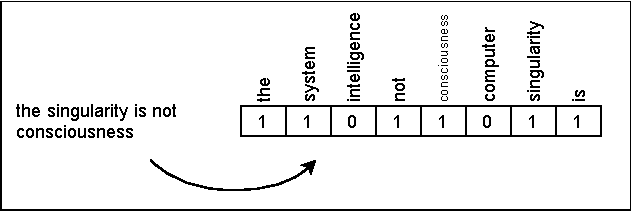
\includegraphics[width=0.8\textwidth]{images/chapters/BOW-TF.pdf}
\end{figure}

From Figure \ref{fig:bow_example}, one may notice, beyond the count of the words from the sample text, there are other words such as \textit{computer}, which did not appear in that text. This happens because the \gls{BOW} creates a position for each word written in the documents. And, as words may appear in some documents and not in others, the representation will not be completely filled, generating sparse and high-dimensional representations. The vocabulary of a set of documents may have thousands of words, while a single document may have only hundreds of words \cite{Witten2011}. Furthermore, sparse and high dimensional representations may degrade the performance of \gls{ML} models and some steps may be taken to improve the representation, such as text preprocessing,  feature selection and dimensionality reduction.

By applying text preprocessing,  one can clean the text and reduce the vocabulary size based on the following \gls{NLP} techniques:

\begin{itemize}[noitemsep]
    \item \textit{Normalization:} converting all characters inside the document to lowercase \cite{Jurafsky2019}.
    \item \textit{Tokenization:} grouping characters in a string into meaningful pieces. This technique identifies important components or tokens using a set of delimiters, such as space and punctuation \cite{Lee1999}.
    \item  \textit{Stemming:} reducing a word variant to its stem by removing any attached suffixes and prefixes (affixes). The stem does not need to be an existing word in the dictionary, but all its variants should map to this form after the stemming has been completed. 
    \item  \textit{Filtering:} removing such terms that do not convey specific meaning (stop words), such as articles, conjunctions, pronouns and prepositions \cite{Kotu2019}.
\end{itemize}


The problem of dimensionality in BOW can be reduced by using dimensionality reduction techniques, such as feature selection and feature projection.
The use of feature selection techniques can improve the text representation and the prediction quality, as discussed in \textcite{Chandrashekar2014} and \textcite{Guyon2003}. Given a set of documents, each of which having $n$ features and the labels for each document, the techniques will define the $k$ most important features to predict the labels. Examples of feature selection techniques include \gls{MI} and \gls{RFE}~\cite{Guyon2003}.

Feature projection techniques can also be used in \gls{BOW} representations. While feature selection techniques select a set of features to represent the data, feature projection techniques transform the data in a high dimensional space to a lower dimensional space, while keeping its characteristics. Examples of techniques for feature projection include \gls{PCA}, \gls{NMF}, and auto-encoders \cite{Jolliffe2016, Guyon2003, Meng2018}. 



Beyond  sparsity and high dimensionality, \gls{BOW} models may not have the sense of order in which the words are written, as it only considers quantitative information from them, and can not detect syntactic and semantic information \cite{Kowsari2019}. Thus, an additional preprocessing step to improve the representation is the extraction of N-grams. Such process consists on grouping words that generally appear together \cite{Kotu2019}. Examples of N-grams include \textit{text mining}, \textit{supreme court}, \textit{special civel court}. One can define the maximum length of N-Grams, however, the higher the length, the bigger the dimensionality of the representation. 


\subsection{Word embeddings}
% Word embeddings
 
    % Trained vs Pre-trained embeddings
    % Word2Vec
    % FastText
    % GloVe




% O que são e qual a Ideia por trás do word embeddings.
Word embeddings, also known as distributed word representations, can capture both the semantic and syntactic information of words while representing them as $n$-dimensional dense vectors. Thus, unlike \gls{BOW}, word embeddings representations are less likely to have the problems of high-dimensionality and sparsity \cite{Lai2016}. 
These representations are generated based on a training process applied to a large unlabeled corpus.

A relevant algorithm is Word2Vec, which uses a neural network to learn to associate words in phrases, and can be divided into two approaches: \gls{SG} and \gls{CBOW}.
In Word2Vec \gls{SG} for instance, the representations are trained as it tries to predict surrounding words in a phrase $w(t-2), ..., w(t+2)$, based on the current word $w(t)$ \cite{Mikolov2013}, as shown in Figure \ref{fig:word2vec_sg}.

\begin{figure}[htb]
    \centering    
    \caption{Word2Vec SG architecture}
    \label{fig:word2vec_sg}
    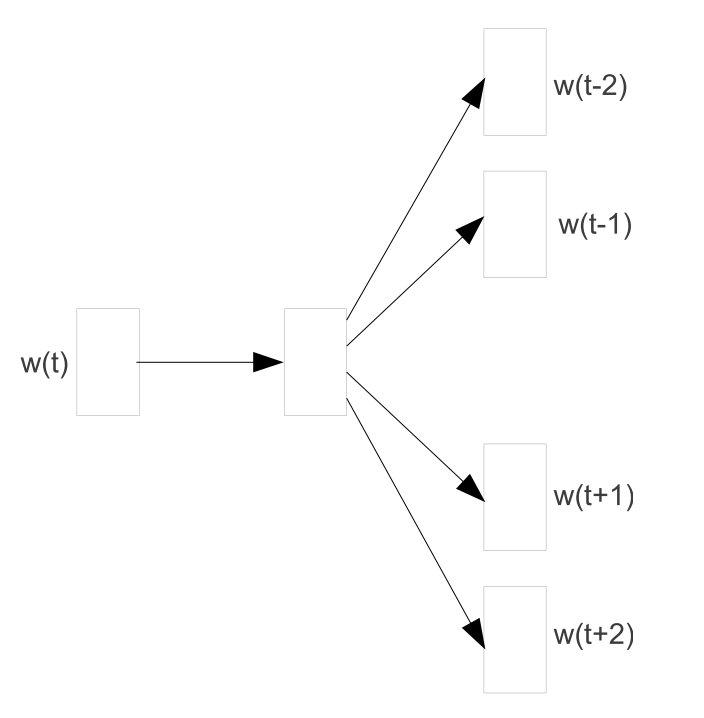
\includegraphics[width=0.5\textwidth]{images/chapters/word2vec_sg.png}
    
    \fonte{\textcite{Mikolov2013}.}
\end{figure}


Although Word2Vec can satisfactorily capture the semantics of words, it will produce distinct representations for the possible variations of the same word. For instance, for the verb \textit{do}, it produces \textit{did}, and \textit{done}. And rare words may not be represented when not contained in the corpus used for training. Thus,  FastText, an algorithm based on Word2Vec, produces representations of words based on the character N-grams, that is, it trains representations for combinations of characters, which then produces the word embeddings~\cite{Bojanowski2016}. 

Another technique for word embeddings generation is GloVe, which creates a co-occurrence matrix containing the frequencies of words in different contexts. Then it applies a dimensionality reduction technique to produce the final representations~\cite{Pennington2014}.


In terms of applications, word embeddings have been  used in many tasks (See Appendix \ref{ap:rsl_representation_law}).  These tasks include clustering~\cite{Mohammed2020}, text classification~\cite{Aggarwal2018} , text summarizing~\cite{Alami2019195}, and others.

Finally, there is an distinction regarding terms for word embeddings.  When the embeddings are used as input for text representation in a pipeline, they are called \textit{pre-trained} representations. The process of creating  the representations has been done before in a unlabeled corpus. However, when such process of training the representation is finished, we call them \textit{trained} representations, as they are the outputs of the pipeline.  

% Finally, there is an distinction regarding terms for word embeddings.  When we apply them as input to \gls{ML} tasks, they are called \textit{pre-trained} representations, since the process of creating  the representations has been done before in a unlabeled corpus. However, when we have just finished such process of training, we call them \textit{trained} representations.  

\subsection{Other representation techniques}

Beyond \gls{BOW}, and word embeddings, there are techniques for text representation proposed recently which can represent semantics, context, order of the text. One example is the \gls{BERT}, a language model that  learns to represent the text in the two directions, that is, from left to right, and vice-versa. The process of training is composed of two steps: pre-training and fine-tuning. The former, the language model is trained over an unlabeled corpus, and in the latter, the representation is fine-tuned for the \gls{ML} task \cite{Devlin2018}.

There is also \gls{ELMo}, a deep contextualized word representation that models both the  syntax and semantics, and how they vary across linguistic contexts. These word vectors are learned functions of the internal states of a deep bidirectional language model, which is pre-trained on a large unlabeled corpus. They can be easily added to existing models and be applied to several tasks, including question answering, textual entailment and sentiment analysis~\cite{Peters2018}.

Finally, the current \gls{SOTA} in text representation is the \gls{GPT-3}, a language model composed of over 175 billion parameters and trained using the openly data available in the internet. \gls{GPT-3} can generate many kinds of texts, such as novels and programming code, and it can be used in tasks like translation and  text summarizing \cite{Brown2020}.
    


%%%%%%%%%%%%%%%%%%%%%%%%%%%%%%%%%%%%%%%%%%%%%%%%%%%%%%%%%
\section{Text Classification}

% Definition and purposes.


Text classification is an important part of \gls{TM} and it has been applied in many contexts \cite{Cardoso2018,Kumar2015,Sheikhalishahi2019}.
In the classification task, we use data to construct a model that learns to relate its features (input) to one of the available  labels (output).
For a given test instance for which the class is unknown, the trained model is used to predict a class label for this instance \cite{Aggarwal2013}.

According to  \textcite{Kowsari2019}, the text classification can follow a pipeline composed of text pre-processing, feature extraction (or text representation), dimensionality reduction (optional), classification models training, and evaluation, as shown in Figure \ref{fig:bow_example}. However, in the Figure there is a step not explicitly mentioned by the author, the train test split.

Techniques for classification can be divided in classical \gls{ML} and \gls{DL}, following the description from Section \ref{sec:basic_definitions}. 
Among classical techniques for classification available, there is the \gls{DT}, which are built based on the induction task in train data, beginning with the root of the tree and proceeding down to its leaves. With the constructed tree, one can make predictions by crossing the tree according to the features from the test data \cite{Quinlan1986}. Other models have been proposed based on \gls{DT}, such as ensemble methods of  \gls{RF}, \gls{GB}, \gls{BG}, and \gls{AB}. An ensemble method tries to improve the performance by training multiple models using distinct approaches according to the techniques mentioned \cite{Breiman2001, Friedman2001, Breiman1996, Schapire1999}.

There is also the \gls{NB} classifier, a computationally inexpensive technique that needs a very low amount of memory. It is based on the Bayes theorem and on the assumption that the attributes are conditionally independent, given the label \cite{Kowsari2019, Pearson1925}.

\gls{LR} is another technique for classification that tries to predict probabilities of the labels \cite{Morgan1988}. There is also \gls{SVM}, which tries to find a hyperplane in an n-dimensional space, where $n$ is the number of features, that distinctly classifies the data points.
\cite{Cortes1995}. 

As the last classical \gls{ML} technique cited in this work, there is \gls{NN} that consists of simple, connected units called neurons, each producing activations. Input neurons are activated base on the input data, other neurons get activated through weighted connections from previously active neurons. The output neurons may influence the environment  \cite{Schmidhuber2015}. 

\gls{DL} techniques, deep neural architectures based on \gls{NN}, have proven to be effective in text classification. Among the techniques available there is \gls{CNN}, which uses convolutional masks to sequentially convolve over the data. For texts, a simple mechanism is to recursively convolve the nearby lower-level vectors in the sequence to compose higher-level vectors. Similar to images, such convolution can naturally represent different levels of semantics shown by the text data \cite{Peng2018}. 

Beyond \gls{CNN} there are sequence based \gls{DL} techniques known as \gls{RNN}, which are networks that make predictions based on the previous states and current input. One relevant kind of \gls{RNN} is the  \gls{LSTM}. Furthermore, the sequence may be one-directional or bi-directional, forming Bi-RNN and Bi-LSTM \cite{Kowsari2019, Hochreiter1997}. 

A recent improvement for sequence based \gls{DL} techniques is the attention mechanism. The \gls{RNN} has the problem of vanish gradient, where it may \textit{forget} what it has learned or seen in the sequence. Thus, attention mechanisms allow the network to focus on distinct parts of the sequence  \cite{Schmidhuber2015}. 
Based on attention mechanisms and in the encoder-decoder architecture, a new type of neural network emerged, i.e., the transformer network. It achieved \gls{SOTA} results in several \gls{NLP} tasks~\cite{Vaswani2017}.

To evaluate the performance of classification models,  the test set is introduced to the models, in order to make  predictions on  unseen data. Then, the predicted outputs are compared to the actual outputs using the evaluation metrics, which may vary for binary and multi-label classifications. To calculate the metrics for classification one can use the confusion matrix, describing the predicted labels in the lines and actual labels in the columns~\cite{Kowsari2019}. Table~\ref{tab:confusion_matrix} shows an example of confusion matrix for a classification task with three labels.

% Confusion matrix aqui

\begin{table}[htb]
\centering
\caption{Confusion matrix example}
\label{tab:confusion_matrix}
\footnotesize
\begin{tabular}{@{}cccc@{}}
\toprule
 & \textbf{Label 1} & \textbf{Label 2} & \textbf{Label 3}  \\ \midrule
\textbf{Label 1} & \textbf{51} & 5 & 1  \\
\textbf{Label 2} & 0 & \textbf{10} & 3  \\
\textbf{Label 3} & 5 & 5 & \textbf{60}  \\ \bottomrule
\end{tabular}
\end{table}

From Table \ref{tab:confusion_matrix}, the example shows the classifier predicted 51 documents as Label 1 where the  actual   label was Label 1. It also predicted three examples as Label 2, where the actual label was Label 3, and so on.

Based on the confusion matrix, one can detect the \gls{TP}, \gls{FP}, \gls{TP}, \gls{TN} and \gls{FN}, as detailed in  \textcite{Kowsari2019} and \textcite{Lever2016}, and calculate the evaluation metrics, as follows.


A simple metric is \textit{accuracy} that indicates the fraction of test instances in which the predicted label matches the actual label, i.e., the sum  of the main diagonal (\gls{TP} + \gls{TN}) in the confusion matrix divided by the number of predictions, following Equation~\ref{eq:accuracy} \cite{Lever2016}.
    
    \begin{equation}
        Accuracy = \frac{TP+TN}{TP+TN+FP+FN}\label{eq:accuracy}
    \end{equation}
    
Another metric is \textit{precision}, that indicates the percentage of instances predicted to belong to the positive label (\gls{TP} and \gls{FP}) that was correct (\gls{TP}), following Equation \ref{eq:precision}. Precision is calculated for each label, having the label to evaluate as the positive label and the others, the negative  \cite{Lever2016}.
    
    \begin{equation}
        Precision = \frac{TP}{TP+FP}\label{eq:precision}
    \end{equation}
    
 \textit{Recall} is the percentage of ground-truth positives (\gls{TP} and \gls{FN}) that have been recommended as positives (\gls{TP}), following Equation \ref{eq:recall}. Recall is also calculated for each label, having the label to evaluate as the positive label and the others, the negative  \cite{Lever2016}.
    
    \begin{equation}
        Recall = \frac{TP}{TP+FN}\label{eq:recall}
    \end{equation}
    
 Finally, there is \textit{F1-Score} is the harmonic mean between the precision and the recall, following Equation \ref{eq:f1_score}.
    
    \begin{equation}
        F1-Score = 2\cdot \frac{Recall\cdot Precision}{Recall + Precision}\label{eq:f1_score}
    \end{equation}


In a multi-label  classification, i.e., when there are more than two labels, the calculus of precision, recall and F1-Score is slightly different. There are three types of calculation: micro, macro and weighted. The first sums the \gls{TP}, \gls{FP}, \gls{FN} for all the labels, and them calculates the metrics. The second calculates the metrics individually for each label and takes the average of those values. The third uses the proportion of examples from each label to calculate an weighted average \cite{Uysal2016}.




%%%%%%%%%%%%%%%%%%%%%%%%%%%%%%%%%%%%%%%%%%%%%%%%%%%%%%%%%
\section{Text Regression}\label{sec:back_regression}



The regression task is a supervised learning approach that, based on samples of pairs $(x,y)$, aims to find a function $f$ that predicts a continuous dependent variable $y$ from $x$ ($y = f(x)$). Since $f(x)$ may not achieve a perfect mapping from $x$ to $y$, there will be some amount of error, which we want to keep as small as possible~\cite{Draper1998}. The representations of $x$ can vary in each context. When applying regression on textual data, $x$ can be books, legal documents, etc.~\cite{Aggarwal2018}.

Based on \textcite{Kowsari2019} and the related work for regression, one can use texts in a regression task to predict one or more dependent variables using the pipeline from Figure~\ref{fig:simple_regression}. Due to the unstructured nature of textual data, some specific steps to apply machine learning in texts are necessary, as we discuss in the following paragraphs~\cite{Aggarwal2018}.


\begin{figure}[htb]
    \caption{Simple regression pipeline}
    \label{fig:simple_regression}
    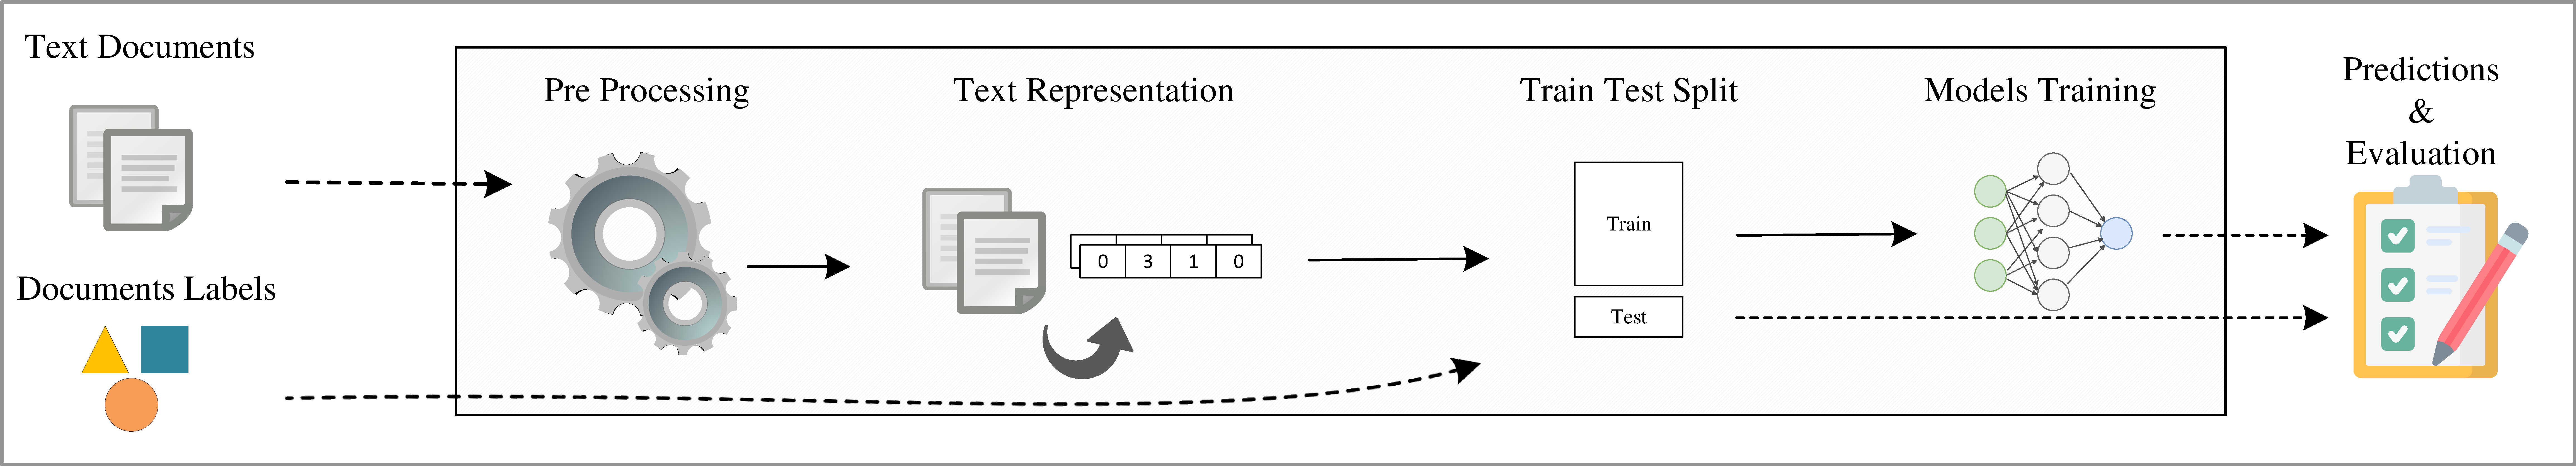
\includegraphics[width=\textwidth]{images/chapters/cap4_simple_pipeline_regression.pdf}
\end{figure}

The pipeline from Figure~\ref{fig:simple_regression} receives as inputs the textual documents and their labels. To prepare this data to further use, some preprocessing operations were applied~\cite{Garcia2015}, which includes tokenization, normalization, filtering, and others~\cite{Lee1999,Jurafsky2019,Kotu2019}.

The next step is to transform the text into a numerical representation which will serve as inputs to regression models. With the numerical representations of the text and their labels, the data can be split into two new datasets: train and test.
%, comprising, for instance, eighty per cent and twenty per cent of the data, respectively. 
Models are trained using the train set and the regression techniques. Using these models, one can make predictions on some continuous output~\cite{Kotu2019}.

Among regression techniques available, there are linear based techniques such as Linear Regression~\cite{Hastie2009} and its derivatives, Ridge~\cite{Hoerl1970}, Elastic Net~\cite{Zou2005} and Lasso~\cite{Tibshirani1996}. And techniques based on \gls{DT}~\cite{Breiman2017} can be used, such as  \gls{RF}~\cite{Breiman2001}, Gradient Boosting~\cite{Friedman2001}, Bagging~\cite{Breiman1996}, AdaBoost~\cite{Schapire1999}, and XGBoosting~\cite{Chen2016}.
Beyond linear and tree-based models, Support Vector Machine~\cite{Drucker1997} and feed-forward Neural Networks~\cite{Kingma2015} can be adapted for the regression task.  

Due to the inner differences among the regression techniques, they can achieve better or worse performances in different situations. Thus, it may be useful to apply some of those models together, so they complement one another. The final prediction of this combination is the average output among the models. This approach is called Ensemble Voting~\cite{Mendes-Moreira2012}.


Focusing again Figure~\ref{fig:simple_regression}, at the final step, the estimation of the prediction quality  of the models on the test set  is carried out using metrics for the regression. A common metric is \gls{RMSE}, which represents the average error of the square differences between the predicted ($y_i$) and the actual ($\hat{y}_i$) values~\cite{Aggarwal2018}, as shown in Equation~\ref{eq:rmse}. This metric is sensitive to outliers and tend to penalize bigger errors, i.e., as the \gls{RMSE} applies a quadratic function on the error, bigger errors have more impact in the final metric~\cite{Chai2014}.

\begin{equation}
    RMSE = \sqrt{\frac{\sum_{i=1}^{n}(y_i - \hat{y_i})^2}{n}} \label{eq:rmse}
\end{equation}

Another metric is the \gls{MAE}, which represents the average of the errors when predicting the dependent variable.  \gls{MAE} is also simple to interpret and it is less sensible to outliers than \gls{RMSE}~\cite{Chai2014}.

\begin{equation}
    MAE = \frac{\sum_{i=1}^{n}|y_i - \hat{y_i}|}{n} \label{eq:mae}
\end{equation}

An additional metric is the coefficient of determination, or $R^2$, interpreted, as shown in Equation~\ref{eq:r2}, as the proportion of observed variation in $y$ that can be explained by the regression model. So, the higher $R^2$, the better the model can explain the variation in $y$~\cite{Devore2011}. $\bar{y}$ represent the mean of the $y$ values.

\begin{equation}
    R^2=1-\frac{\sum_{i=1}^{n}(y_i-\hat{y}_i)^2}{\sum_{i=1}^{n}(y_i - \bar{y})^2} \label{eq:r2}
\end{equation}

Acceptable values of error and  coefficient of determination  may depend on the domain's requirements and the range of possible values for the dependent variable \cite{Zhou2011, Torres2005}.



